% !Mode:: "TeX:UTF-8"%確保文檔utf-8編碼
\documentclass[border=2pt]{standalone}
\usepackage{tikz}
\usepackage{pgfplots}
\pgfplotsset{compat=newest}
\usetikzlibrary{intersections,calc,positioning,backgrounds}


\begin{document}

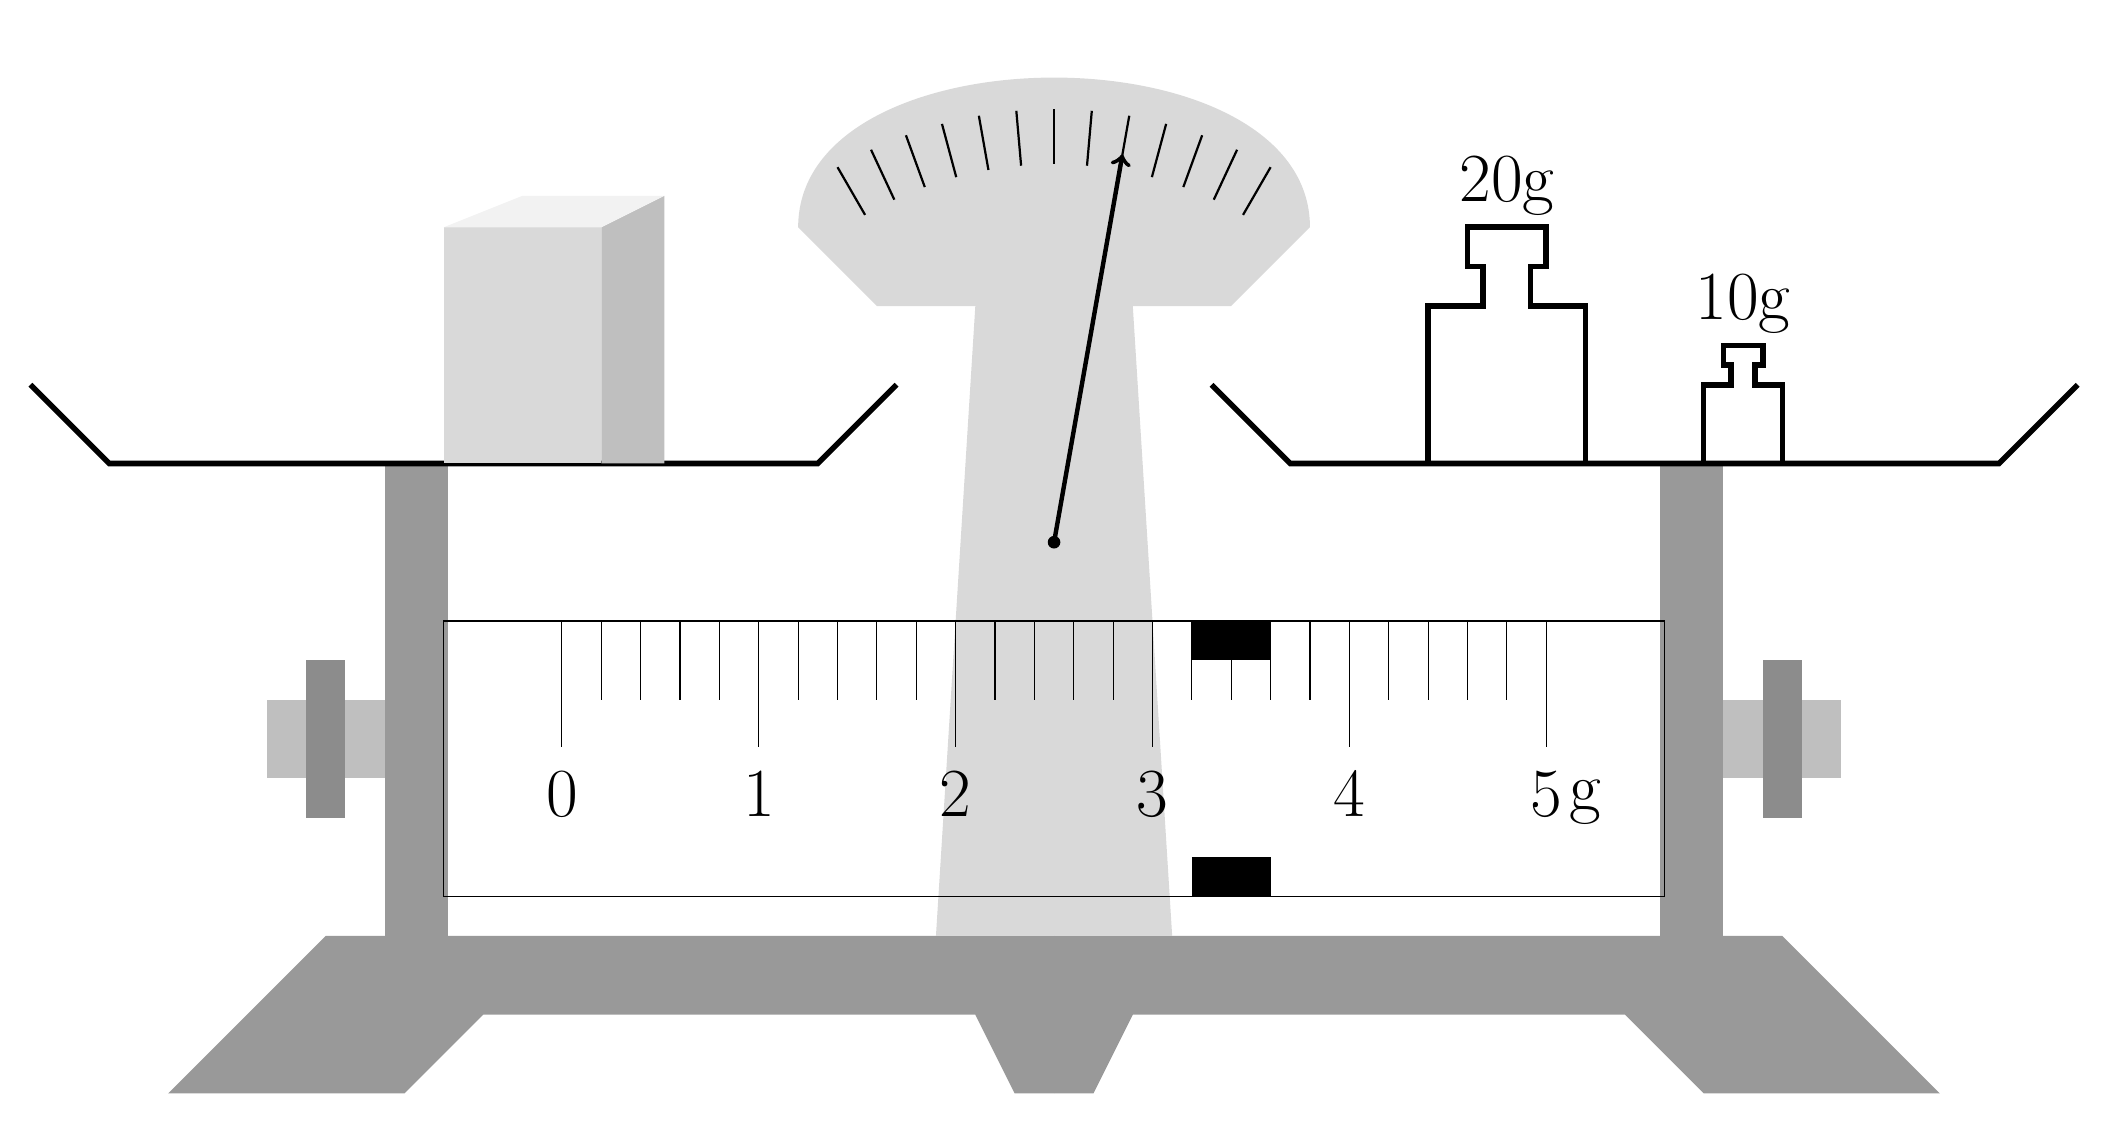
\begin{tikzpicture}


%刻度尺
\begin{scope}[xscale=0.5]

%显示的数值多少g
\def\gnum{3.2}
\pgfmathsetmacro{\gmove}{10*\gnum/2}
%主线轴
\def\startx{0}
\def\endx{25}
\pgfmathsetmacro{\stepx}{\startx+1}
\pgfmathsetmacro{\stepxfive}{\startx+5}
\pgfmathsetmacro{\stepxten}{\startx+10}

\coordinate (startpoint) at (\startx,0) ;
\coordinate (endpoint) at (\endx,0) ;
\draw [](startpoint) -- (endpoint);

\draw ($(startpoint) + (-3,-3.5)$) rectangle ($(endpoint) + (3,0)$);

%细小刻度
\foreach \x in {\startx,\stepx,...,\endx}
  \draw [](\x,0) -- (\x,-1);   

%5分之一刻度
%\foreach \y in {\startx,\stepxfive,...,\endx}
%  \draw [] (\y,-1.6) -- (\y,0);


%10分之一刻度
\foreach \i in {\startx,\stepxfive,...,\endx}
  \draw [] (\i,-1.6) -- (\i,0)
  node[below=1.8cm] {\Huge \pgfmathprint{int(\i/5)}};

%unit
\node at ($(endpoint) +(1,-2.3)$) {\Huge  g};


%额外的修改
\draw[line width =0.5cm,yshift=-0.25cm] (\gmove,0)-- +(2,0);
\begin{scope}[yshift=-3cm]
\draw[line width =0.5cm,yshift=-0.25cm] (\gmove,0)-- +(2,0);
\end{scope}

\end{scope}

%刻度尺之外的修改
\begin{pgfonlayer}{background}

\begin{scope}[xshift=6.25cm,yshift=-4cm,xscale=1]
\fill[gray!80] (0,0) -- (6.25,0) -- ++(3,0) -- ++(2,-2) -- ++(-3,0) -- ++(-1,1) -- (1,-1) -- (0.5,-2) -- (0,-2)  ;
\fill[gray!30] (0,0)-- (1.5,0) -- (1,8)-- (0,9) ;
\fill[gray!50] (7.7,2) rectangle (10,3);
\fill[gray!90] (9,1.5) rectangle (9.5,3.5);
\fill[gray!80] (7.7,0) rectangle (8.5,6);
\draw[line width=2pt] (2,7)--(3,6) -- (12,6)--(13,7);
\end{scope}


%反对称
\begin{scope}[xshift=6.25cm,yshift=-4cm,xscale=-1]
\fill[gray!80] (0,0) -- (6.25,0) -- ++(3,0) -- ++(2,-2) -- ++(-3,0) -- ++(-1,1) -- (1,-1) -- (0.5,-2) -- (0,-2)  ;
\fill[gray!30] (0,0)-- (1.5,0) -- (1,8)-- (0,9) ;
\fill[gray!50] (7.7,2) rectangle (10,3);
\fill[gray!90] (9,1.5) rectangle (9.5,3.5);
\fill[gray!80] (7.7,0) rectangle (8.5,6);
\draw[line width=2pt] (2,7)--(3,6) -- (12,6)--(13,7);
\end{scope}

\end{pgfonlayer}

%简单非定量表盘
\fill (6.25,1) circle (0.08);
\fill[gray!30] (8.5,4) -- ++(1,1)  to[out=90,in=90]  ++(-6.5,0) -- +(1,-1);

\begin{scope}[xshift=6.25cm,yshift=1cm]
\foreach \x in {60,65,...,120} \draw[thick] (\x:5.5) -- (\x:4.8);
\end{scope}

\draw[ultra thick,->] (6.25,1) -- ++(80:5);

%砝码1
\begin{scope}[xshift=12cm,yshift=2cm]
\draw[line width=2pt] (0,0) node[above=3cm] {\Huge 20g} -- (1,0) -- (1,2) -- (0.3,2) -- (0.3,2.5) -- (0.5,2.5) -- (0.5,3)--(0,3);
\begin{scope}[xscale=-1]
\draw[line width=2pt] (0,0) -- (1,0) -- (1,2) -- (0.3,2) -- (0.3,2.5) -- (0.5,2.5) -- (0.5,3)--(0,3);
\end{scope}
\end{scope}

%砝码2
\begin{scope}[scale=0.5,xshift=30cm,yshift=4cm]
\draw[line width=2pt] (0,0) node[above=1.5cm] {\Huge 10g} -- (1,0) -- (1,2) -- (0.3,2) -- (0.3,2.5) -- (0.5,2.5) -- (0.5,3)--(0,3);
\begin{scope}[xscale=-1]
\draw[line width=2pt] (0,0) -- (1,0) -- (1,2) -- (0.3,2) -- (0.3,2.5) -- (0.5,2.5) -- (0.5,3)--(0,3);
\end{scope}
\end{scope}

%待测物体
\begin{scope}[xshift=-1.5cm,yshift=2cm]
\fill[gray!30] (0,0) rectangle (2,3);
\fill[gray!50] (2,0) -- (2.8,0.0) -- (2.8,3.4) -- (2,3);
\fill[gray!10] (0,3)-- (1,3.4) -- (2.8,3.4) -- (2,3);
\end{scope}


\end{tikzpicture}


\end{document}